\documentclass[tikz,border=2pt]{standalone}
\usepackage{tikz}
\usetikzlibrary{arrows.meta,calc}

\definecolor{roadgray}{RGB}{211,214,216}
\definecolor{curbdark}{RGB}{86,91,94}
\definecolor{curblight}{RGB}{139,145,148}
\definecolor{egocolor}{RGB}{65,145,162}
\definecolor{targetcolor}{RGB}{232,112,58}
\definecolor{nominalcolor}{RGB}{0,139,151}

% The vehicle drawing is the one used by the ego--obstacle dynamics
% figure, scaled by 0.44 so that its 2.10-unit body length matches the
% 0.924-unit footprint of this scene. The fourth argument steers the
% front wheels. The vehicle longitudinal axis is the local positive x
% direction.
\newcommand{\drawvehicle}[4]{%
    \begin{scope}[shift={(#1)},rotate=#2,scale=0.44]
        % Wheels sit under the body, so they are drawn first.
        \path[fill=black!76]
            (-0.73,-0.60) rectangle (-0.30,-0.43)
            (-0.73,0.43) rectangle (-0.30,0.60);
        \begin{scope}[shift={(0.515,-0.515)},rotate=#4]
            \path[fill=black!76]
                (-0.215,-0.085) rectangle (0.215,0.085);
        \end{scope}
        \begin{scope}[shift={(0.515,0.515)},rotate=#4]
            \path[fill=black!76]
                (-0.215,-0.085) rectangle (0.215,0.085);
        \end{scope}
        \path[
            fill=#3!82,
            draw=black!72,
            line width=0.45pt,
            rounded corners=1.2pt
        ] (-1.05,-0.48) rectangle (1.05,0.48);
        \path[
            fill=white!72!#3,
            draw=black!48,
            line width=0.25pt
        ] (-0.34,-0.37) -- (0.20,-0.37) -- (0.42,-0.27)
          -- (0.42,0.27) -- (0.20,0.37) -- (-0.34,0.37) -- cycle;
        \path[
            fill=black!10,
            draw=black!45,
            line width=0.25pt
        ] (-0.79,-0.34) rectangle (-0.48,0.34);
        \path[fill=white!90!#3,draw=black!45,line width=0.25pt]
            (0.79,-0.27) -- (1.00,0) -- (0.79,0.27) -- cycle;
    \end{scope}%
}


\begin{document}
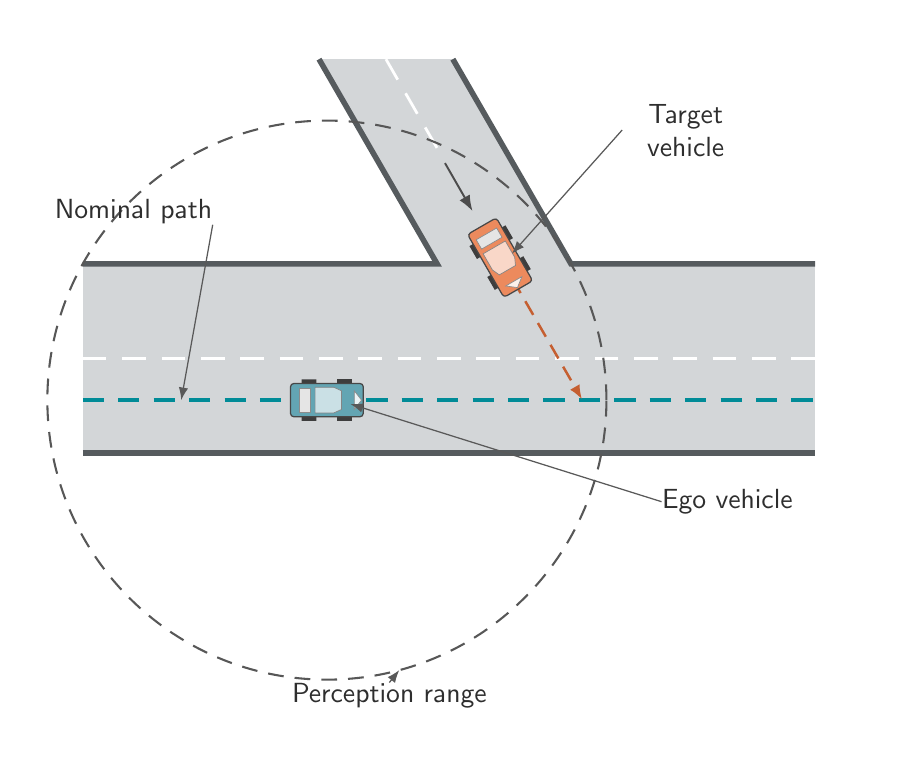
\begin{tikzpicture}[
    callout/.style={font=\sffamily\normalsize,align=center,text=black!82,inner sep=0pt},
    leader/.style={-{Latex[length=1.6mm,width=1.2mm]},draw=black!65,line width=0.45pt}
]
\path[use as bounding box] (-5.45,-4.90) rectangle (5.45,4.20);
\coordinate (egoVehicle) at (-1.65,-0.53);
\coordinate (targetVehicle) at (0.55,1.28);
\def\sensingradius{3.55}

% The oblique side road joins the main road ahead of the eastbound ego.
\path[fill=roadgray] (-4.75,-1.20) rectangle (4.55,1.20);
\path[fill=roadgray] (-0.25,1.20) -- (1.45,1.20)
    -- (-0.05,3.80) -- (-1.75,3.80) -- cycle;
% Curb segments stop at the side-road mouth.
\draw[curbdark,line width=2.0pt] (-4.75,-1.20) -- (4.55,-1.20);
\draw[curbdark,line width=2.0pt] (-4.75,1.20) -- (-0.25,1.20) -- (-1.75,3.80);
\draw[curbdark,line width=2.0pt] (-0.05,3.80) -- (1.45,1.20) -- (4.55,1.20);
% Lane markings are interrupted at the side-road mouth.
\draw[white,line width=1.0pt,dash pattern=on 3mm off 2mm]
    (-4.75,0) -- (4.55,0);
\draw[white,line width=1.0pt,dash pattern=on 3mm off 2mm]
    (-0.90,3.80) -- (-0.25,2.67);
% The nominal route belongs to the ego lane.
\draw[nominalcolor,line width=1.25pt,dash pattern=on 2.7mm off 1.8mm]
    (-4.75,-0.53) -- (4.55,-0.53);
% The complete dashed circle is centered exactly at the ego-vehicle center.
\draw[draw=black!66,line width=0.75pt,dash pattern=on 2mm off 1.4mm]
    (egoVehicle) circle[radius=\sensingradius];
% A short projected target path meets the ego nominal path ahead.
\draw[-{Latex[length=1.8mm,width=1.4mm]},draw=targetcolor!85!black,
    line width=0.9pt,dash pattern=on 2mm off 1.2mm]
    (targetVehicle) -- (1.59,-0.52);
\drawvehicle{egoVehicle}{0}{egocolor}{0}
\drawvehicle{targetVehicle}{-60}{targetcolor}{0}
\draw[-{Latex[length=2mm,width=1.5mm]},draw=black!70,line width=0.7pt]
    (-0.15,2.48) -- (0.20,1.87);

\node[callout,anchor=west,text width=16mm] (targetLabel) at (2.10,2.90) {Target\\vehicle};
\draw[leader] (targetLabel.west) -- ($(targetVehicle)+(0.15,0.05)$);
\node[callout,anchor=west] (egoLabel) at (2.60,-1.82) {Ego vehicle};
\draw[leader] (egoLabel.west) -- ($(egoVehicle)+(0.30,-0.05)$);
\node[callout,anchor=east] (pathLabel) at (-3.10,1.86) {Nominal path};
\draw[leader] (pathLabel.south east) -- (-3.50,-0.53);
\node[callout,anchor=west] (rangeLabel) at (-2.10,-4.28) {Perception range};
\draw[leader] (rangeLabel.north) -- ($(egoVehicle)+(285:\sensingradius)$);
\end{tikzpicture}
\end{document}
